	
	\begin{enumerate}[label=\alph*)]
		\item La resisitividad, como hemos visto a lo largo de todos los ejericcios, viene dada por:
		\begin{equation}
			\rho = \frac{1}{q(\mu_n n + \mu_p p)}
		\end{equation}
		Por lo que solo tenemos que calcular $n$ y $p$ para $\mu_n$ y $\mu_p$ dados (valores que tendremos que coger de otro ejercicio). Así pues, obtenemos $n$ y $p$ a partir de las ecuaciones:

		\begin{equation}
			n = n_i e^{(E_F-E_i)/kT} \qquad p = n_i e^{(E_i-E_F)/kT}
		\end{equation}
		Donde conocemos $N_C$ y $N_V$ a 300K (temperatura ambiente) y la diferencia de $E_c-E_F=E_g/4$ y $E_F-E_v=3E_g/4$ en $x>W/2$ (véase diagrama de bandas). Así pues conocemos los valores:

		\begin{equation}
			n= 7.91\times 10^{14} \ \cm^{-3} \tquad p = 4.5\times 10^{14} \ \cm^{-3}
		\end{equation}
		Usando las siguientes movilidades (calculadas con las ecuacioens de portadores mayoritarios/minoritarios previas):
		
		\begin{equation}
			\mu_n = 1290 \ \cm^2 /  \text{V s} \tquad \mu_p = 499 \ \cm^2 /  \text{V s}
		\end{equation}
		tal que la resistividad en $W/2<x$:

		\begin{equation}
			\rho = 5.02 \ \Omega \cm
		\end{equation}
		\textcolor{red}{Da 7.73. En gneral hacen aproximaciones ignorando uno de los portadores.} Ahora solo queda calcualar la energía cinética mínima $T_{\min}$ que deben tener. Como podemos ver la energía de la banda de conducción aumenta de la región $x>W/2$ a la región $x<W/2$. Así pues:

		\begin{equation}
			T_{\min} = E_c(-W/2) - E_c(W/2) = E_g/2 = 0.506 \	 \eV
		\end{equation}
		\item Como sabemos el campo eléctrico viene dado por:
		\begin{equation}
			\Ecal = \frac{1}{q} \derivadas{E_i}{x}
		\end{equation}
		y el potencial $V(x)=-E_i(x)+V_0$ donde $V_0$ es una constate arbitraria que nos ayuda a redefinir el cero del potencial. Como para calcular la derivada (y $V_0$ siempre nos permite redefinir el cero de $V$) solo necesitamos conocer la \textit{dependencia de $E_i$ con la posición}, podemos escribir

		\begin{equation}
			E_i = E_{i0} - \frac{E_g}{2} \frac{x}{W}
		\end{equation}
		siendo $E_{i0}$ una constante irrelevante que contiene información de la energía respecto al cero $E_F=0$ eV. Así pues:

		\begin{equation}
			\Ecal = - \frac{1}{q} \frac{E_g}{2W}
		\end{equation}
		Así pues:

		\begin{equation}
			V=V_0 + \frac{E_g}{q} \frac{x}{2W}
		\end{equation}
		Para ver si está en equilibrio termodinámico tenemos que ver si $J_n=J_p=0$. Veamos que $J_n=0$ implica que:

		\begin{equation}
			J_n = J_n |_{\text{difusion}} +J_n |_{\text{arrastre}} = q\mu_n n \Encal + qD_n\derivadas{n}{x} = 0
		\end{equation}
		De tal modo que, si estamos en equilibrio se tiene que verificar que
		\begin{equation}
			\Ecal_n = \frac{D_n}{\mu_n} \frac{1}{n} \derivadas{n}{x} =
			\frac{kT}{q} \frac{1}{n} \derivadas{n}{x}
		\end{equation}
		donde hemos aplicado las reglas de Einstein (válido para el equlibrio y fuera del equlibrio). Ahora solo tenemos que evaluar $n(x)$ y su derivada. Es sencillo de ver que la única dependencia mostrada en el diagrama de bandas:

		\begin{equation}
			n = \left\lbrace
			\begin{array}{ll}
				N_c e^{-\frac{1}{kT}\frac{3E_g}{4}}	& \text{si} \ x<-W/2 \\
				N_c e^{-\frac{1}{kT}\frac{E_g}{4} \parentesis{\frac{-x+W}{W/2}}}	& \text{si} \ -W/2<x<W/2 \\
				N_c e^{-\frac{1}{kT}\frac{E_g}{4}} & \text{si} \ W/2<x
			\end{array} \right.
		\end{equation}
		De lo cual deducimos que la derivada es:

		\begin{equation}
			\derivadas{n}{x} = \left\lbrace
			\begin{array}{ll}
				0	& \text{si} \ x<-W/2 \\
				\frac{1}{kT}\frac{E_g}{4}\frac{2}{W}N_c e^{-\frac{1}{kT}\frac{E_g}{4} \parentesis{\frac{-x+W}{W/2}}}	& \text{si} \ -W/2<x<W/2 \\
				0 & \text{si} \ W/2<x
			\end{array} \right.
		\end{equation}
		Consecuentemente el campo eléctrico:

		\begin{equation}
			\Ecal_n = - \frac{1}{q} \frac{E_g}{2W}   \qquad \text{si} \ - W/2<x<W/2
		\end{equation}
		Que como podemos ver es la misma expresión. Para los portadores huecos se puede llegar a lo mismo siguiendo los mismos pasos (la única diferencia es que aparecen dos signos menos que se cancelan). Veamos como quedan las gráficas:

		\begin{center}
			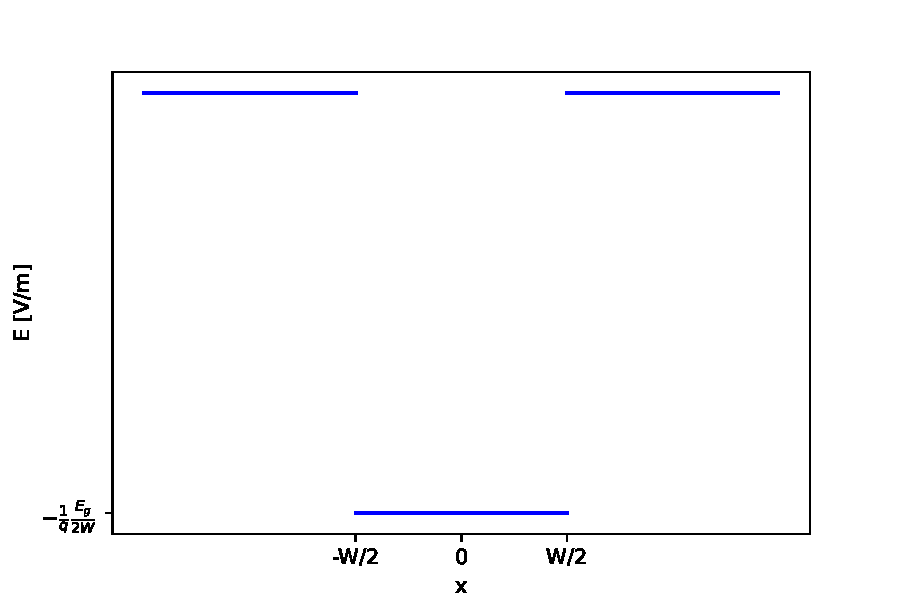
\includegraphics[width=0.7\linewidth]{Cuerpo/Ch_02/02_Ejercicio_15_E(x).pdf}
		\end{center}
		\begin{center}
			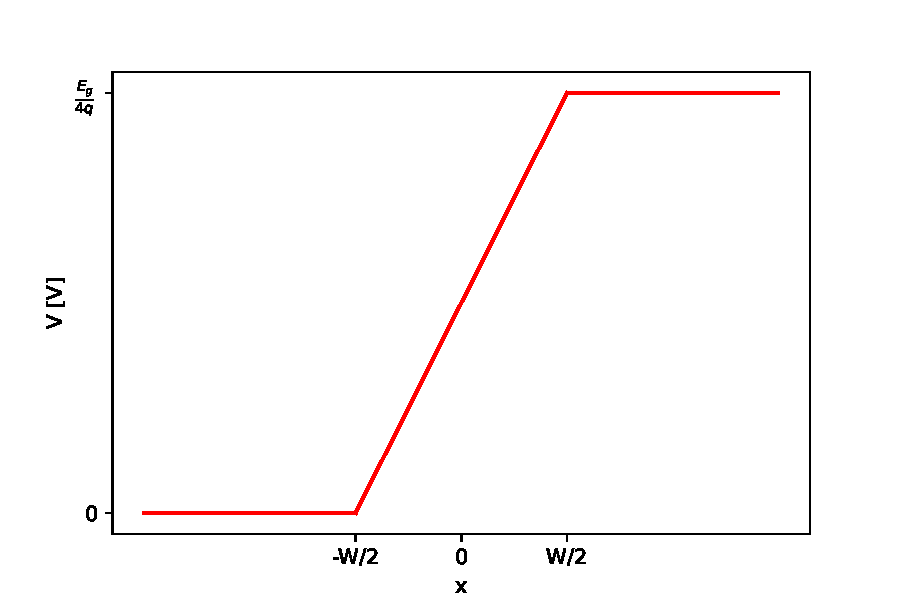
\includegraphics[width=0.7\linewidth]{Cuerpo/Ch_02/02_Ejercicio_15_V(x).pdf}
		\end{center}

		\item Respondemos a cada una de las preguntas:
		\begin{itemize}
			\item La densidad de corriente de electrones y de huecos en $x=0$ es cero, como hemos visto en el apartado anterior. De otra manera no estaríamos en el equilibrio termodinámico.
			\item Corriente de arrastre hay, ya que el campo eléctrico no es nulo (en $x=0$). Así pues:
			\begin{equation}
				\Jn_n |_{\text{arrastre}} = q \mu_n n \Encal =  - \mu_n \frac{E_g}{2W} N_c  e^{-\frac{1}{kT}\frac{E_g}{2}}  \hnx
			\end{equation}
			Lógicamente la corriente de arrastre tiene que tener la misma dirección que la corriente eléctrica, ya que aún que la velocidad del electrón tendrá la dirección contraria al campo eléctrico y la corriente de carga tendrá la dirección contraria a la velocidad del electrón.
			\item Corriente de difusión hay, y en virtud de que $\Jn_n|_{\text{arrastre}}=- \Jn_n|_{\text{difusion}}$, tenemos que
			\begin{equation}
				\Jn_n |_{\text{arrastre}} = - q \mu_n n \Encal =  \mu_n \frac{E_g}{2W} N_c  e^{-\frac{1}{kT}\frac{E_g}{2}}  \hnx
			\end{equation}
		\end{itemize}
	\end{enumerate}
